\section{Introduction}
\label{sec:introduction}

Many web user interfaces implement security-critical functionality. Examples include web-based configuration of safety-critical devices like Programmable Logic Controllers (PLCs) used in manufacturing plants, medical devices, and home automation systems~\cite{7306669,siemens,siemens2,schneider}. Payments in online banking and cryptocurrency transactions from online wallets are additional examples of security-critical user interfaces implemented as web services. Figure~\ref{fig:PLC} shows on the left a configuration web form for a commercial PLC system~\cite{controlbyweb} that we use as a running example throughout this chapter and on the right a browser-based Bitcoin wallet provided by BitGo~\cite{bitgo}. The defining characteristics of such web services are that (i) they accept input from the user, (ii) the inputs are sensitive to minor changes, and (iii) after committing an input, the resulting action is difficult to reverse.

%In such remote configuration, the communication between the host and the safety-critical device (or its programmer device) is easy to protect through standard means such as a TLS connection~\cite{dierks2008transport}. However, if the host platform gets compromised---as standard PC platforms so often do---the adversary can manipulate any user-provided configuration settings. Such \emph{user input manipulation attacks} are difficult to detect (before it is too late!) and can have serious consequences, including safety violations that can put human lives in danger.

Typically in such web services, the communication between the host and the remote server (e.g., PLC, banking service, online wallet) is easy to protect through standard means such as a TLS connection~\cite{dierks2008transport}. However, if the host platform gets compromised---as standard PC platforms so often do---the adversary can manipulate any user-provided input. Such \emph{user input manipulation attacks} are difficult to detect (before it is too late!) and can have serious consequences, including safety violations that can put human lives in danger and financial loss. 
%In the context of social media post (such as Facebook, twitter, reddit etc.), manipulated post often leads to misleading post, fake news, rumors etc~\cite{gordon,fitzpatrickmedia,lee2013crowdturfers,ferrara2015manipulation}. 

More generally, trusted input through an untrusted host platform to a remote server remains an open problem despite various research efforts~\cite{sgxio,utp,x86,wimpyKernel,gyrus,weigold2011}. Indeed, all known approaches for \emph{trusted input} have their limitations. For example, financial transaction confirmation from the display of a separate trusted device, like a USB dongle, is prone to user habituation and requires expensive additional hardware \cite{weigold2011}. Secure input systems based on a trusted hypervisor have a large TCB and do not tolerate complete host compromise \cite{sgxio}. We review such prior solutions and their limitations further in Section~\ref{sec:problemStatement}.

% \begin{figure}[t]
%   \centering
%     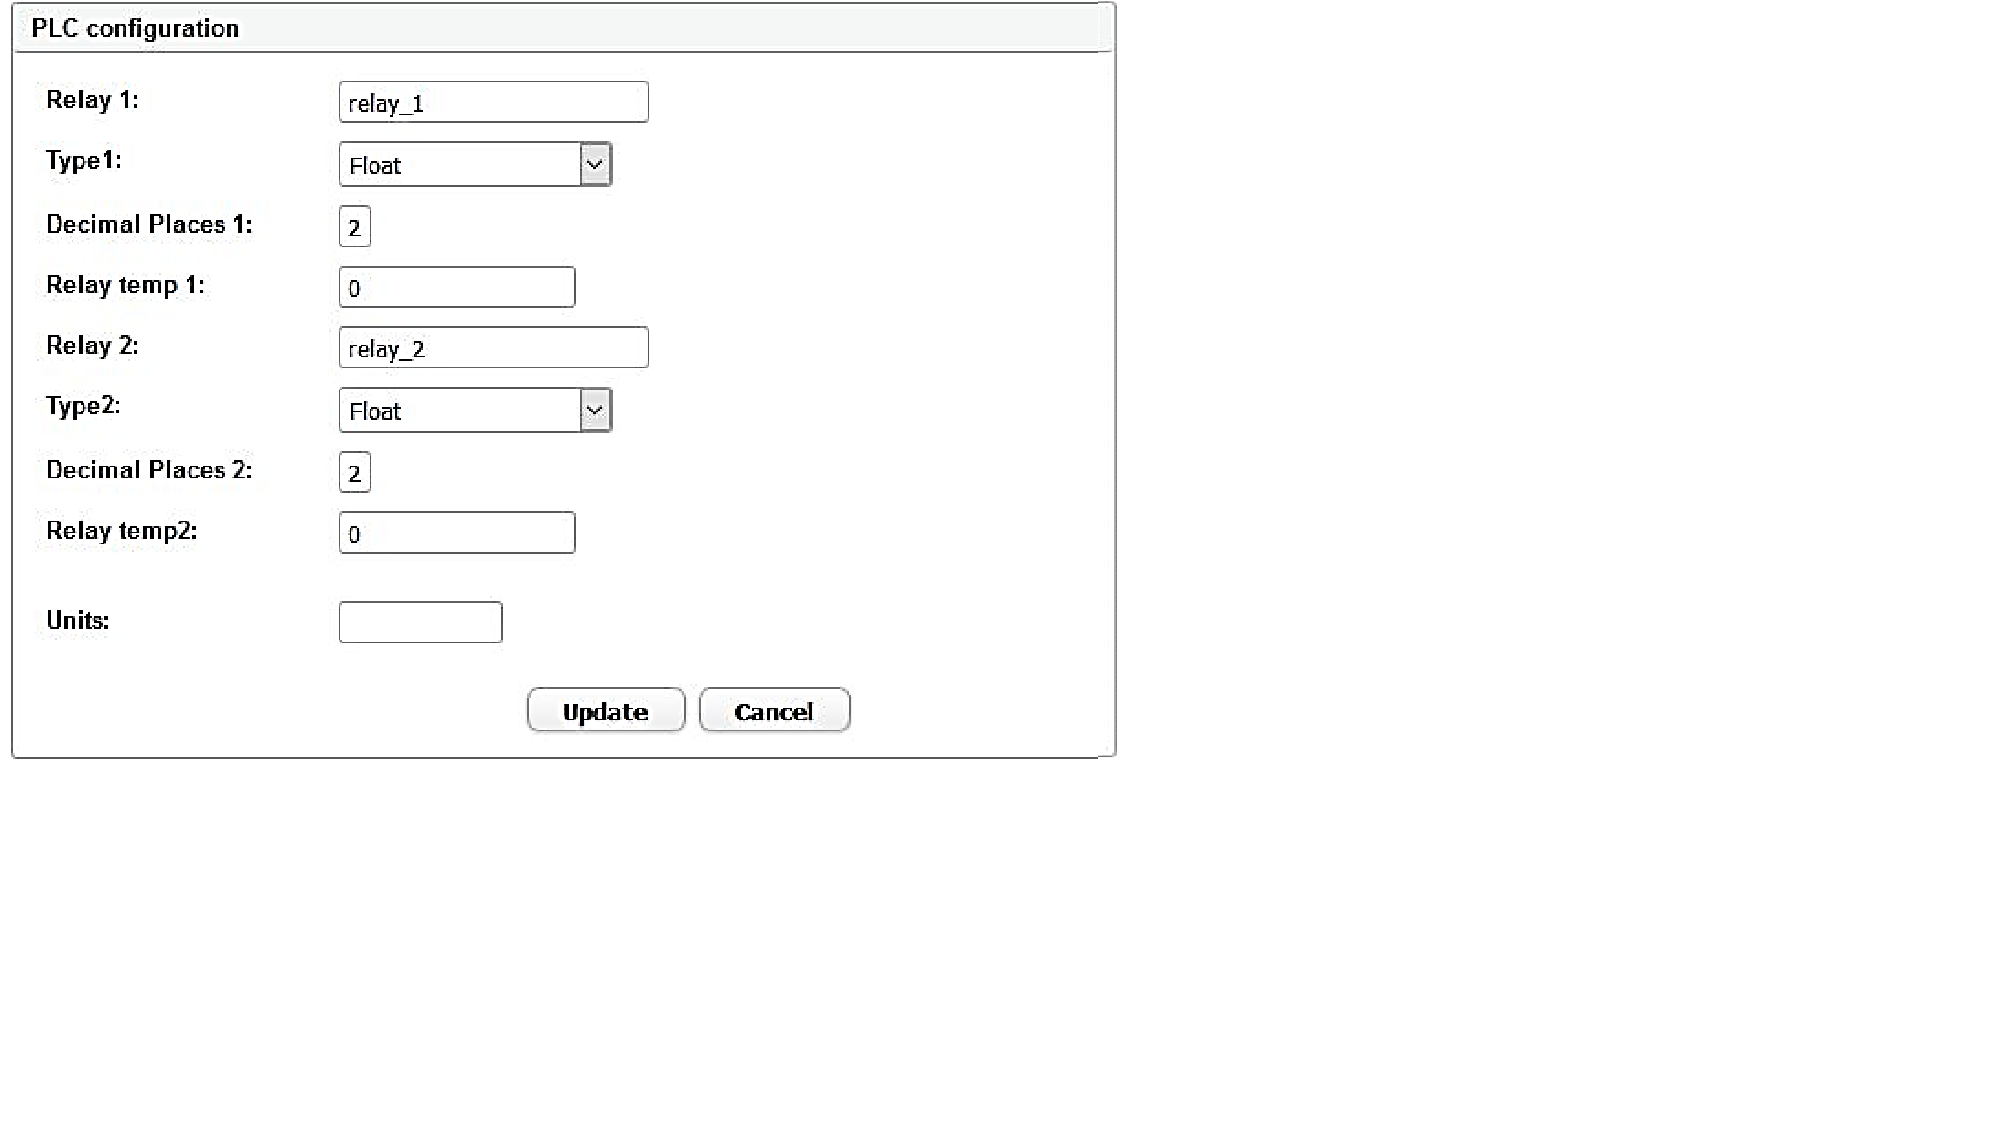
\includegraphics[trim={0 6cm 14cm 0},clip,width=\linewidth]{PLC_revised.pdf}
%     \caption{\textbf{Example configuration page.} Screenshot from the ControlByWeb x600m~\cite{controlbyweb} I/O server configuration page.}
%     \vspace{-20pt}
%     \label{fig:PLC}
% \end{figure}


\begin{figure}[t]
  \centering
    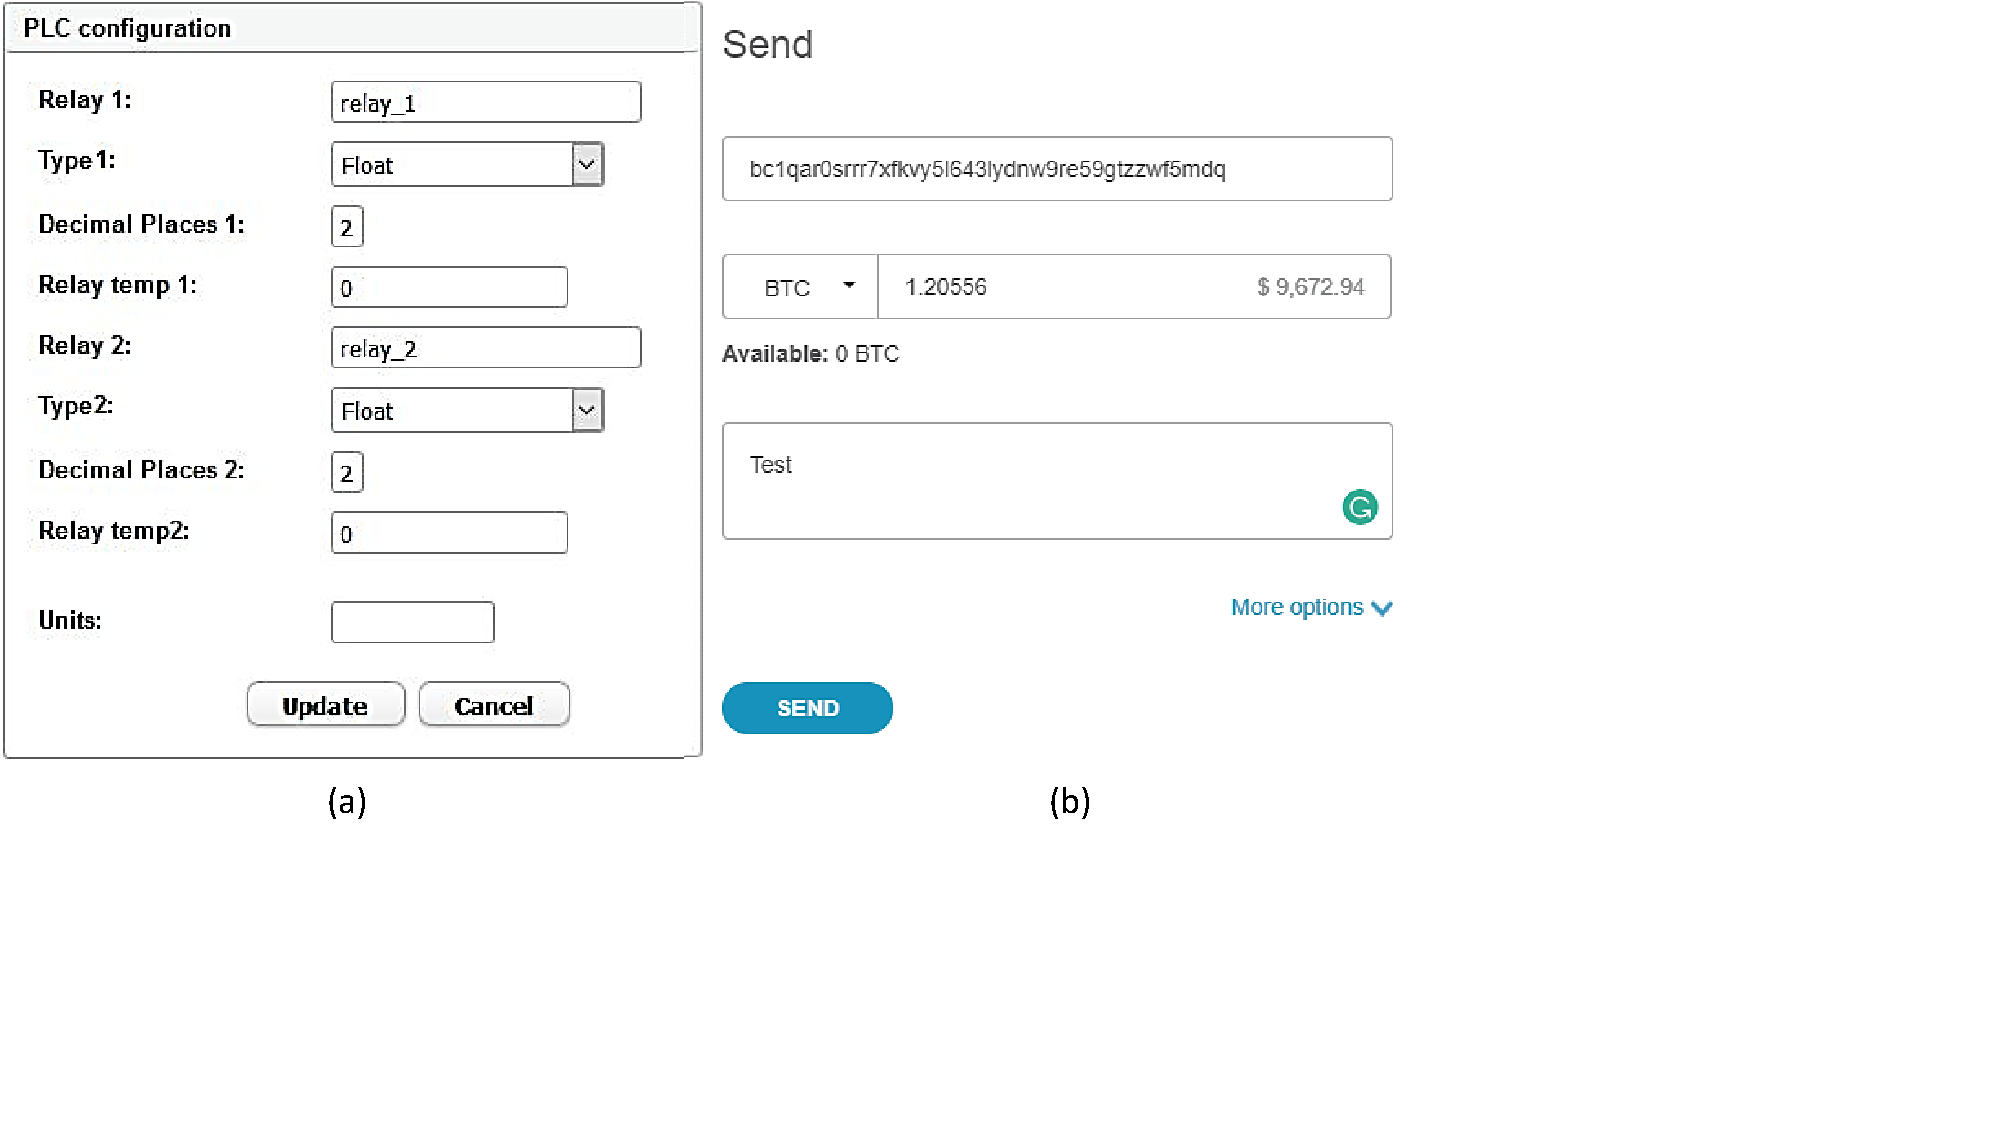
\includegraphics[trim={0 4cm 10cm 0},clip,width=\linewidth]{chapters/IntegriKey/images/config_pages.pdf}
    \caption[Example configuration page of a web-based PLC]{\textbf{Example configuration page of a web-based PLC.} Screenshot from the (a) ControlByWeb x600m~\cite{controlbyweb} I/O server configuration page, (b) web-based bitcoin wallet provide by BitGo~\cite{bitgo}. In rest of this chapter, we use the PLC server as the running example for our proposed system.}

    \label{fig:PLC}
\end{figure}


\subsection{Our Solution} 

In this chapter, we address the \emph{integrity protection} of user input in security-critical web user interfaces. Our goal is to design a solution that provides strong protection (e.g., no risk of user habituation, small TCB) and easy adoption (e.g., minimal changes to the existing systems and user experience, low deployment cost). We use remote configuration of a commercial safety-critical device (see Figure~\ref{fig:PLC} (a)) as a running example, but we emphasize that our solution is not limited to that application domain. In Section~\ref{sec:discussion_IK} we discuss how the same approach can be applied to integrity protection of various other services including financial transactions, social media posts, and email.

The basic idea behind \name is straightforward and we call this approach \emph{input trace matching}.  When the user needs to perform a security-critical web operation like configuring a PLC device or performing a cryptocurrency payment, he installs a trusted embedded device between the user input peripheral and the host platform. This device intercepts user's input events, passes them through to the host, and sends a trace of them (over a secure channel) to an authenticated remote server that compares the trace to the user input received from the host to detect input manipulation. Once the user has completed the web transaction, he can remove the embedded device from the host to preserve the user's privacy and to prevent that any subsequent input events are sent to the same server unnecessarily.

This approach can be seen as a second-factor for user input integrity protection. If the primary protection mechanism (i.e., the integrity of the host platform itself) fails, the secondary protection provided by input trace matching ensures that the target safety-critical device cannot be misconfigured.

Secure and easy adoption of this idea involves overcoming some technical challenges. The first is related to security, as an adversary that fully controls the host can execute restricted forms user input manipulation attacks, where he exchanges input values from interchangeable UI elements (e.g., two integers with overlapping ranges). Such \emph{swapping attacks} cannot be detected by the server relying on the input trace alone. Another challenge is related to deployment. Our trusted device needs to communicate with the server, but we want to avoid building an (expensive) separate communication channel into it. We further want to avoid the need to install additional software on the host that could assist in such communication. 


\myparagraph{System and tool} Based on this idea, we design and implement \name, a user input integrity protection system, that is tailored for \emph{keyboard} input, as keyboard input is sufficient for controlling many security-critical web interfaces including configuration of existing commercial safety-critical devices and execution of financial transactions.

Our system realizes the trusted embedded device as a simple USB bridge (for short \device) that is accompanied by a server-side user input matching library. To prevent subtle swapping attacks, our solution includes a simple \emph{user labeling} scheme, where the user is asked to annotate interchangeable input elements. For easy adoption, we leverage the recently introduced WebUSB browser APIs to enable communication between \device and the server in a plug-and-play manner. 

We also develop \tool, a user-interface analysis tool that helps developers to protect their web services and minimizes the added effort of users. In particular, the \tool detects input fields in web forms that require labeling and annotates the UI accordingly. 

We implemented a prototype of \device using an Arduino board and evaluated \tool using a range of existing web-based configuration UIs supported by x600m, a commercial PLC server~\cite{controlbyweb}, and several web-based Bitcoin wallets such as Bitgo~\cite{bitgo}, Bitcoin wallet~\cite{bitcoinwallet}, Coinbase~\cite{coinbase}, Coinspace~\cite{coin} and Blockchain wallet~\cite{blockchain}. Our results show that the tool can correctly process the configuration UIs of many existing security-critical web user interfaces. Our \device implementation adds a delay of $5$ ms on the processing of keyboard events and its TCB is 2.5 KLOC. 

We also conducted a preliminary user study where we simulated a swapping attack on $15$ study participants. Labeling prevented the attack in $14$ cases.


\subsection{Our Contributions} To summarize, in this chapter we make the following contributions:

\begin{enumerate}
    %\item \emph{New approach for integrity protection.} We propose input trace matching as a novel approach for integrity protection of user input on untrusted host platforms.
    \item \emph{New attack.} We identify swapping attacks as a novel form of user input manipulation against simple user input matching strategies.
    \item \name. We design and implement a user input integrity protection system that is tailored for keyboard input, prevents swapping attacks, and is easy to deploy.
    \item \tool. We develop a user interface analysis and webpage annotation tool that helps developers to protect their web services and minimizes user effort.
    \item \emph{Evaluation.} We verified that our tool can process UIs of existing safety-critical systems and cryptocurrency wallets correctly. Our experiments show that the performance delay of \name user input integrity protection is low. Our preliminary user study indicates that user input labeling prevents swapping attacks in most cases.
   %, and our preliminary user study indicates that user can perform the needed labeling. 
\end{enumerate}


\subsection{Organization of this Chapter} The rest of the chapter is organized as the following. We explain our problem in Section~\ref{sec:problemStatement_IK}. Section~\ref{sec:ourApproach} introduces our approach, Section~\ref{sec:integriKey} describes our system and Section~\ref{sec:integriTool} the UI analysis tool. We provide security analysis in Section~\ref{sec:securityAnalysis_IK}. Sections~\ref{sec:implementation_IK} and~\ref{sec:results} explain our implementation and evaluation. In Section~\ref{sec:discussion_IK} we discuss other applications for our solution. Section~\ref{sec:relatedWork_IK} reviews related work and Section~\ref{sec:conclusion_IK} concludes this chapter.



